\section{Dataset Details}
\subsection{Training Dataset}

The primary pretraining corpus in our experiments is Colossal Clean Crawled Corpus (C4), a curated English text dataset comprising over 170 billion tokens. This corpus is derived from CommonCrawl, a common practice in the pretraining of LLMs \cite{brown2020language,raffel2020exploring,touvron2023llama}. This data source is also prominently featured in openly available LLM pretraining corpora, including The Pile \cite{gao2020pile} and RedPajama \cite{together2023redpajama}.
 There are different versions of CommonCrawl data and our selection of C4 for pretraining is driven by driven by its size and quality.

 We also compare with pre-training on the Refined Web corpus \cite{penedo2023refinedweb}.  The dataset is also derived from the CommonCrawl, however has a more stringent filtering process. Our selection of Refined Web is for comparing synthetic rephrases to high quality subsets of web data, which were shown to achieve similar performance compared with curated datasets \cite{penedo2023refinedweb}.  For our experiments we used the first $3050$ files and train for 300B tokens to match training on C4.  We aso conduct experiments with the first 1650 files to account for multiple epochs on the Refined Web dataset.  

\subsection{Pile Perplexity Evaluation}
For the evaluation phase, we employed 20 subsets from the Pile corpus. We excluded the Europarl subset because it contained non-English language. The subsets used are:
CC, StackExchange, Wikipedia, GitHub, PubMed Abstracts, Openwebtext2, Freelaw, Math, NIH, USPTO, Hackernews, Enron, Books3, PubMed Central, Gutenberg, Arxiv, Bookcorpus2, Opensubtitles, Youtubesubtitles, Ubuntu, and Philpapers. We take the first 10000 samples from each subset and split into documents of maximum length 1024.  The reported average in all perplexity plots is a weighted average over the perplexity of all domains according to the ratios in Table~\ref{tab:ratios}.  

\subsubsection{Pile Weighted Average Ratios}

We report the ratios for samples according to the first 10,000 documents from our Pile validation set in Table~\ref{tab:ratios}.  Note that there are some slight variations in the ratios compared with those reported in \citep{gao2020pile}, but most ratios are similar.
\begin{table}
    \centering
    \begin{tabular}{lcc}
    \toprule
       Dataset  & Validation Ratio (\%) & Published Ratio (\%) \\\hline
       ArXiv  & 10.4 & 9.0\\
       BookCorpus2 & 0.8 & 0.8\\
       Books3 & 11.8 & 12.1\\
       Pile-CC & 14.0 & 18.11\\
       Enron & 0.1 & 0.1\\
       EuroParl & 1.1 & 0.7\\
       FreeLaw & 5.3 & 6.1\\
       Github & 10.9 & 7.6\\
       Gutenberg & 1.5 & 2.2\\
       Hackernews & 0.6 & 0.6\\
       Dm Mathematics & 2.0 & 1.2\\
       NIH & 0.2 & 0.3\\
       OpenSubtitles & 1.3 & 1.6\\
       OpenWebText2 & 8.2 & 10.0\\
       PhilPapers & 0.7 & 0.4\\
       PubMed Abstracts & 0.7 & 3.1\\
       PubMed Central & 14.9 & 14.4\\
       StackExchange & 5.8 & 5.1\\
       Ubuntu & 1.3 & 0.9\\
       USPTO & 2.7 & 3.7\\
       Wikipedia & 3.4 & 1.5\\
       YoutubeSubtitles & 0.6 & 0.6\\
       \bottomrule
    \end{tabular}
    \caption{Pile ratios for our evaluation compared with published ratios}
    \label{tab:ratios}
\end{table}

\subsection{Zero-shot Evaluation Dataset}
We evaluate our models on a total of 13 different zero-shot benchmarks to assess their abilities across various natural language tasks. These benchmarks are categorized into two subsets: Specialized Knowledge and General Understanding.

\paragraph{Specialized Knowledge}
This subset comprises datasets that focus on domain-specific knowledge and expertise.

\begin{itemize}
\item \textbf{ARC Challenge (ARC-C)}: This dataset is part of the AI2 Reasoning Challenge (ARC)~\citep{allenai:arc}, containing science exam questions from grades 3 to 9. The ARC Challenge set includes more difficult questions that necessitate higher-order reasoning.
\item \textbf{SciQ}: A dataset of science exam questions, specifically designed to evaluate the ability of NLP models in understanding and reasoning within the scientific domain~\citep{SciQ}.
\item \textbf{PubMedQA}: This dataset focuses on biomedical literature and is designed to evaluate the understanding of medical and healthcare-related information~\citep{jin2019pubmedqa}.
\item \textbf{MathQA}: This dataset challenges models in mathematical problem-solving, requiring both numerical understanding and reasoning skills~\citep{amini-etal-2019-mathqa}.
\item \textbf{MMLU}: Multi-domain question answering, MMLU assesses the model's expertise over a wide range of specialized subjects, from professional domains to academia~\citep{hendryckstest2021}.
\end{itemize}

\paragraph{General Understanding}
This subset contains datasets that test general cognitive skills, language understanding, and common sense reasoning.

\begin{itemize}
\item \textbf{ARC Easy (ARC-E)}: The Easy set of the AI2 Reasoning Challenge~\citep{allenai:arc} features questions from the same source as ARC-C but are considered less challenging and do not require as advanced reasoning skills.
\item \textbf{BoolQ}: A dataset consisting of boolean (yes/no) questions, focusing on reading comprehension and general understanding of natural language text~\citep{clark-etal-2019-boolq}.
\item \textbf{Winogrande (Wino.)}: This dataset challenges models on common sense reasoning in a language context, focusing on pronoun disambiguation tasks~\citep{ai2:winogrande}.
\item \textbf{PIQA}: Physical Interaction Question Answering tests the understanding of everyday physical processes, an aspect of practical common sense~\citep{Bisk2020}.
\item \textbf{HellaSwag}: This dataset evaluates a model's ability to complete scenarios in a contextually and logically coherent manner, requiring both language understanding and common sense reasoning~\citep{zellers2019hellaswag}.
\item \textbf{TruthfulQA}: Focused on the generation of truthful, accurate answers, this dataset challenges models on their ability to discern and reproduce factually correct information~\citep{lin2021truthfulqa}.
\item \textbf{OpenBookQA (OBQA)}: OpenBookQA requires understanding a wide array of facts and concepts, thereby evaluating the model's broader knowledge and reasoning skills~\citep{OpenBookQA2018}.
\item \textbf{LogiQA-2}: This dataset involves logical reasoning, testing the model's capability to understand and apply logical constructs and principles~\citep{logiqa2}.
\end{itemize}

Each dataset in these subsets is carefully selected to challenge and evaluate specific aspects of natural language processing models, ranging from domain-specific knowledge in science, medicine, and mathematics, to broader skills like common sense reasoning and general language understanding.



\section{Filtering Details for Synthetic Data}
When generating synthetic paraphrases using language models, we occasionally encounter the challenge of extraneous introductions in the generated outputs. Such paraphrases might commence with phrases like "Here's a paraphrase...", "The following..." or even contain keywords such as "high-quality English". To mitigate this, we've developed a method to filter and refine the synthetic outputs.

\subsection{Methodology}

The primary function, \texttt{remove\_unwanted\_part}, starts by splitting the input data into individual sentences. If the first sentence contains delimiters such as "\textbackslash n\textbackslash n" (indicating a new paragraph) or ":", the function checks the segment preceding the delimiter for the aforementioned unwanted elements. If these elements are detected, the preceding segment is removed. The entire revised content is then reconstructed and returned. In cases where no modifications are applicable, but we still have the flagged keywords, we remove the paraphrase completely. To achieve this: 

\begin{enumerate}
    \item Split the input data into individual sentences using the NLTK's sentence splitter function.
    \item Examine the first sentence for the presence of delimiters.
    \item If a delimiter is detected, check the preceding segment for unwanted elements.
    \item If unwanted elements are found, discard the preceding segment (before an occurrence of \texttt{"\textbackslash n\textbackslash n"} or \texttt{":"}).
    \item Modify and return the filtered paragraph.
\end{enumerate}

Based on manual inspection we found that the error rate (occurrence of sentences with unwanted elements) after the modification is less than 0.1\%. 







\section{Properties of Synthetic Corpus}
\label{sec:synth_properties}
To understand the properties of synthetic data generated from the rephrase model that lead to better pre-training performance, we compare the semantic similarity, syntactic complexity, and diversity between synthetic data, C4 data, and data from the Pile.  Our primary focus is answering the following questions about synthetic data: (i) Do models trained on synthetic data perform better due to information leakage from the rephrase model? (ii) Does the rephrase model accurately capture multiple styles? (iii) What attributes of synthetic data make it high quality? Our investigation helps address what data is beneficial for better generalization to specific domains, and quantify the importance of data variability and quality.

\subsection{Experimental Setup}
We take a subset of the first 1000 documents from each of the datasets.  For synthetic comparisons with real C4 data, we take pairs of samples, while for Pile subsets, we take the first 1000 samples from the test subset. When computing dataset quality statistics, we remove outliers more than two standard deviations in metric value.  When the number of samples from the Pile subset was fewer than 1000, we split samples. Figures with distributions use a Gaussian Kernel Density Estimator (KDE) to construct distributions for statistics from 1000 values.



\subsection{Semantic Properties}

\begin{figure*}
  \centering
 
    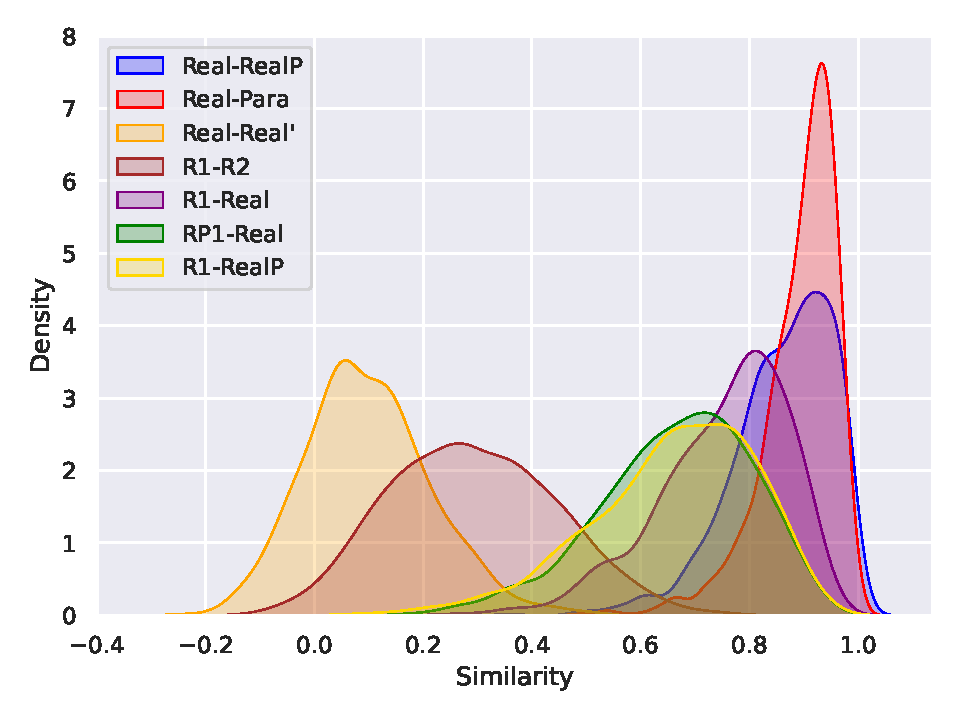
\includegraphics[width=4.5in]{figures/mrpc_cosine_sim_comparison.pdf}
    \caption{Cosine similarity medium synthetic MRPC rephrases}

  \label{fig:cosine_sim_mrpc_style}
\end{figure*}

In Section~\ref{sec:ablations}, we compared pairs of examples of synthetic and real data to confirm the performance gain is not attributed to knowledge leakage from the rephrase models using a pre-trained BERT model trained with SimCSE objective \citep{gao2021simcse} for medium and qa prompts in  Figure~\ref{fig:cosine_sim_style}(a)  and (b).  We additionally compare the similarity of synthetic rephrases and actual rephrases using the MRPC corpus in Figure~\ref{fig:cosine_sim_mrpc_style}(c).  We denote this additional comparison by RealP (real paraphrase), while maintaining comparison of splits of the sentence: R1 and R2.  Synthetic rephrases have similar cosine similarity on average and lower spread compared with true rephrases according in the MRPC corpus.

\begin{figure*}
  \centering
  \begin{subfigure}{0.45\linewidth}
    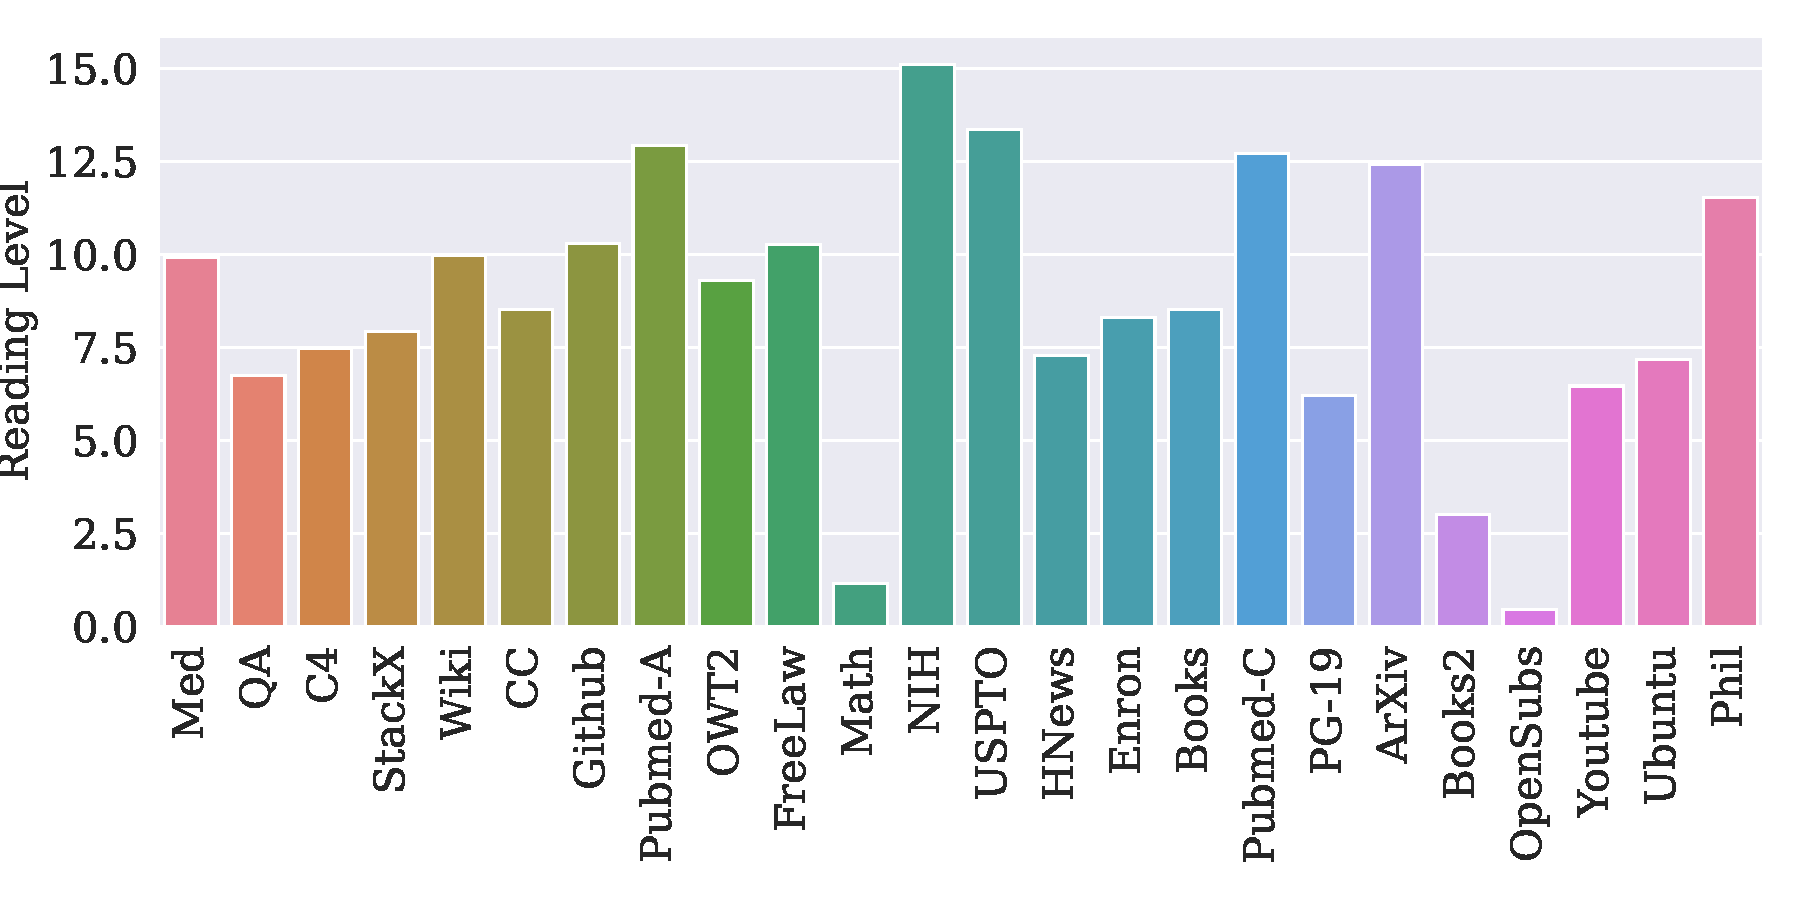
\includegraphics[width=\columnwidth]{figures/read_scores.pdf}
    \caption{Flesch-Kincaid Reading Level}
  \end{subfigure}
  \hfill
  \begin{subfigure}{0.45\linewidth}
      
\includegraphics[width=\columnwidth]{figures/diversity.pdf}
        \caption{Type token ratio}
  \end{subfigure}
  \caption{Comparison of readability and diversity (ttr) of synthetic data compared with C4 and different subsets of the Pile.}
  \label{fig:readability}
\end{figure*}

As the semantic information is similar between C4 and our synthetic data, we further investigate stylistic differences in the data. Figure~\ref{fig:readability}(a) shows the Flesch–Kincaid reading levels for different rephrase styles, and the Pile.  Our findings indicate that C4 is on the low end of reading level (7-8).  In contrast,  medium increases the reading level to 10, and qa synthetic variants further reduces the reading level to 6.  Medium synthetic data matches the reading level of Wikipedia, and other high reading level datasets yielding better performance on these domains. On QA synthetic data, we observe reduced reading level. This is because we observed that sentences are typically split into question and answer leading to shorter setnences compared with in the original text and medium style rephrases.  This leads to lower metric values for many of the metrics. For type token ratio, we note that the diversity is quite similar between medium and most subsets of the Pile.  The QA dataset has particularly low TTR matching ubuntu, github, and math as these are more similar to QA format datasets and have heavy repetition of the Question, and Answer format.

\subsection{Syntactic Properties}
\begin{figure*}
  \centering
  \begin{subfigure}{0.45\linewidth}
    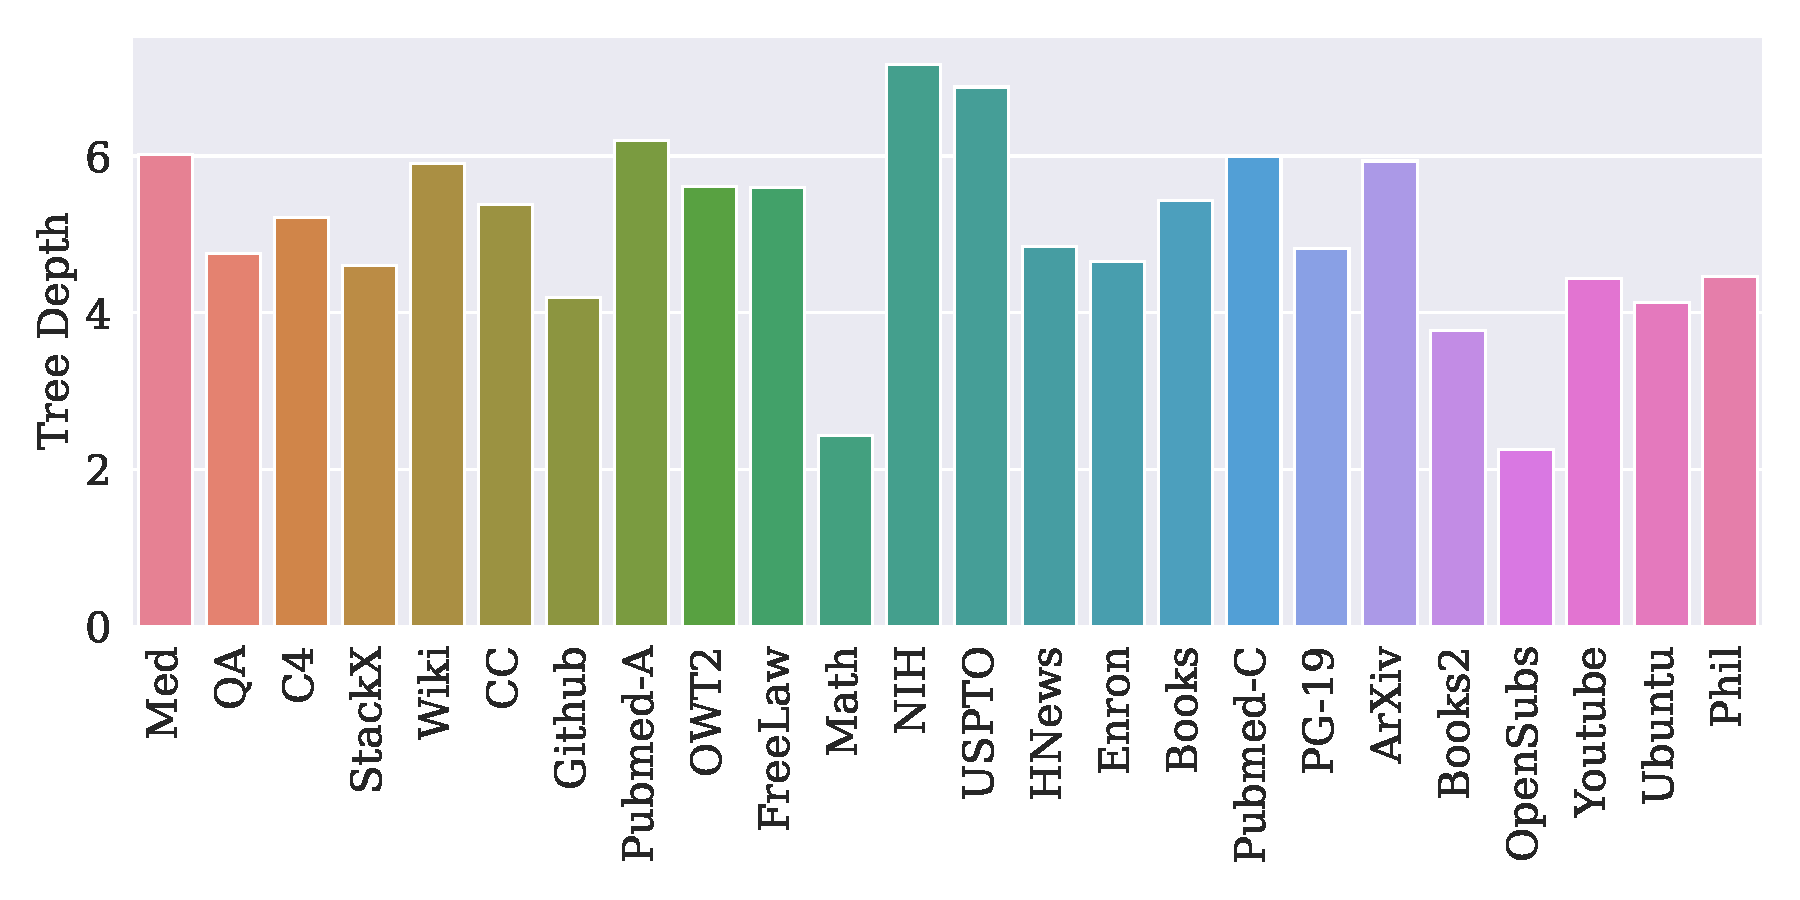
\includegraphics[width=\columnwidth]{figures/depth.pdf}
    \caption{Tree Depth}
  \end{subfigure}
  \hfill
  \begin{subfigure}{0.45\linewidth}
    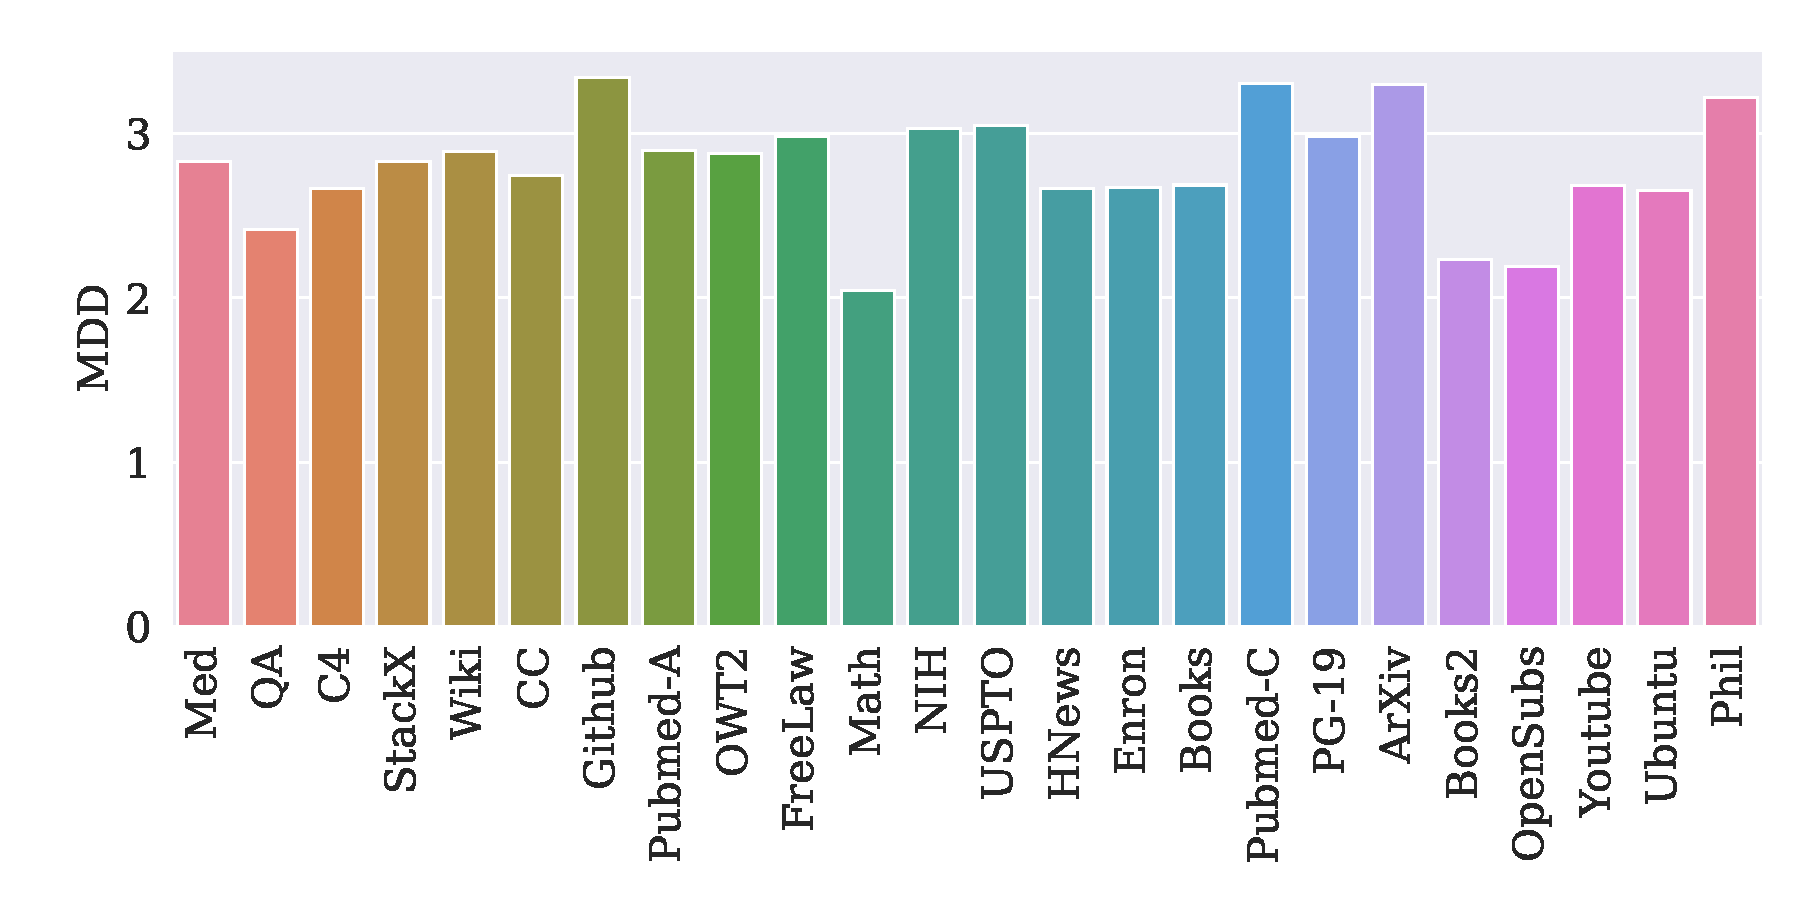
\includegraphics[width=\columnwidth]{figures/dist.pdf}
    \caption{Mean Dependency Distance}
  \end{subfigure}  
  \caption{Comparison between synthetic and real data from the C4 corpus showing that synthetic data have higher syntactic complexity indicated by higher average tree depth, and higher mean dependency distance (MDD).}
  \label{fig:syntactic_complexity}
\end{figure*}

Finally, we compare the mean tree depth (measured by the mean over setences of the depth of the dependency tree),  and mean dependency distance (measured as the average dependency distance of any pair of words within a sentence) in Figure~\ref{fig:syntactic_complexity}, which have been shown to be good measures of syntactic difficulty \cite{futrell2015large,gibson2000dependency,oya2021three}.    We find similar trends as for reading level and TTR diversity where mediums tyle increase depth, mdd, and syntactic complexity in general.  We find again that QA style reduces this complexity.













































\section{Evaluation Metrics}\label{app_eval}

The metric utilized for evaluation is the \textit{macro token level perplexity}. Given a batch of encoded texts, the perplexity at the token level was computed as follows:

Given the accumulated loss over the entire dataset, denoted as \( L \), and the total number of tokens, represented by \( T \), the macro token-level perplexity, denoted as \( \mathcal{P} \), is calculated as:

\begin{equation}
\mathcal{P} = \exp\left(\min\left(20, \frac{L}{T}\right)\right)
\end{equation}

Where:
\begin{itemize}
    \item \( \exp \) is the exponential function.
    \item \( L \) is the cumulative loss over all shifted logits and labels in the dataset.
    \item \( T \) is the total number of tokens in the dataset.
\end{itemize}

The value of 20 acts as an upper limit to stabilize the metric in cases of high loss values.



\section{Additional Results for Smaller Model and Token Sizes}

\subsection{Results for 350M Models Trained for 75B Tokens}

 \begin{figure}[t]
    \centering
    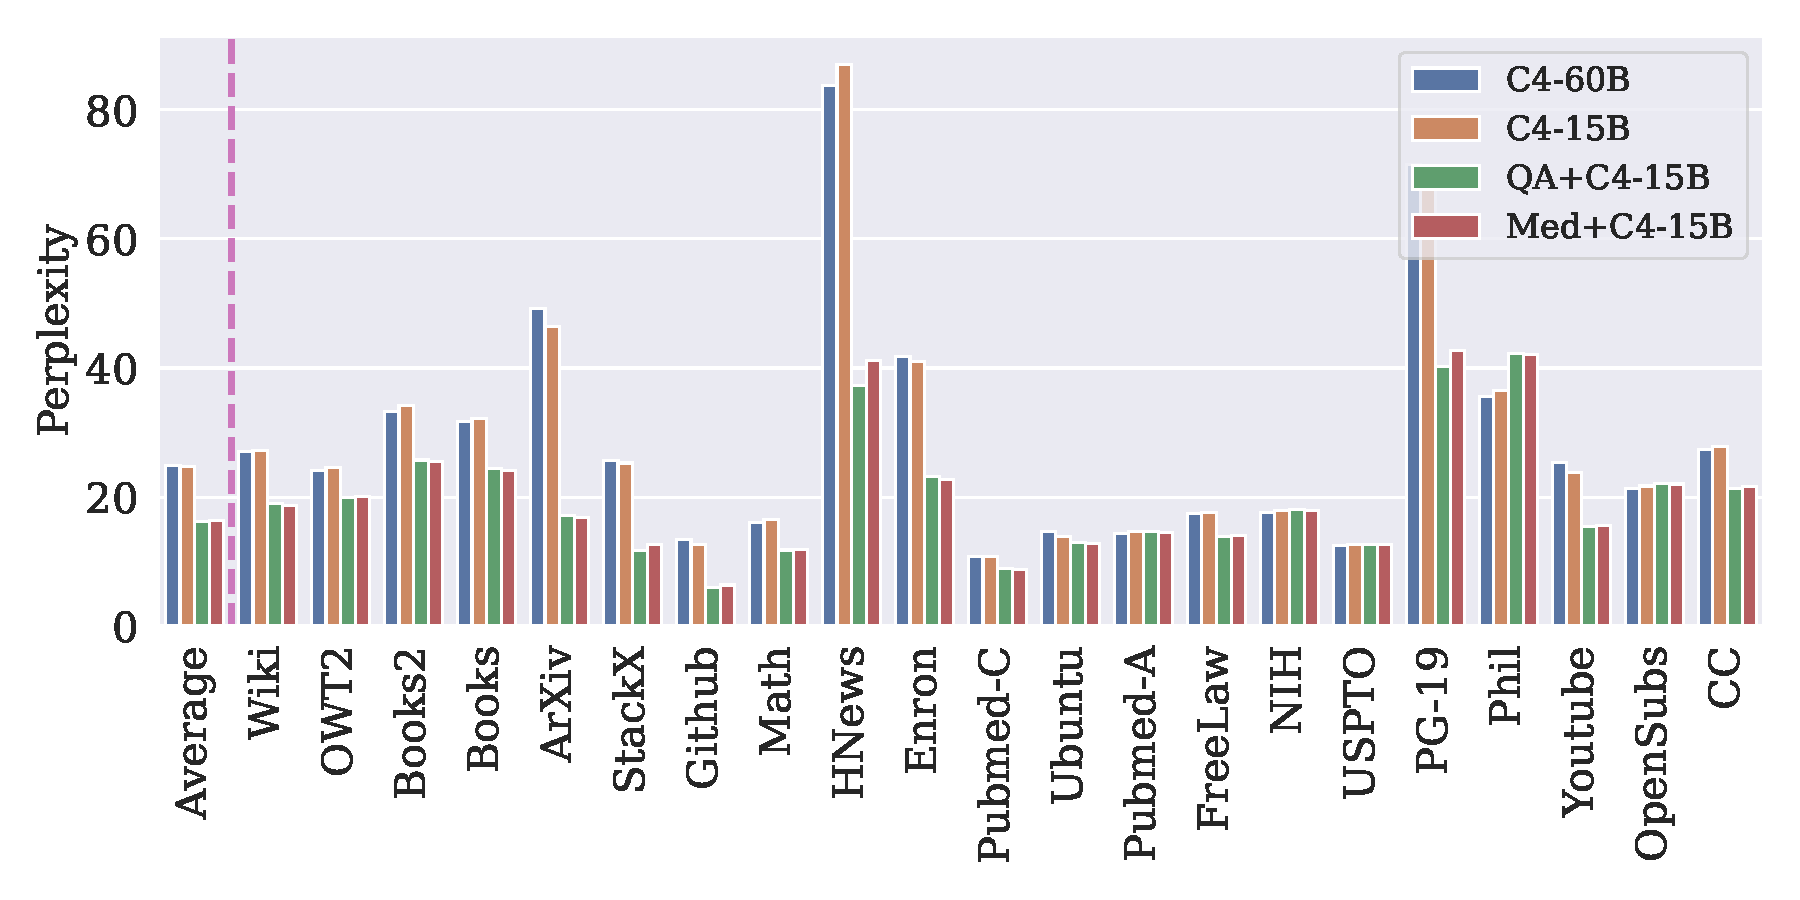
\includegraphics[width=\linewidth]{figures/all_pile_style_345M_75k.pdf}
    \caption{Perplexity across all domains of the Pile comparing combining multiple styles of synthetic data.  Models are 350M parameters trained for a total of 75B tokens.}
    \label{fig:350M_75K}
\end{figure}

\begin{table*}[t]
    \centering
    \scalebox{0.8}{
    \begin{tabular}{lccccc>{\columncolor{LightCyan}}c}
        \toprule
        Dataset (Real Tok.) & ARC-C & SciQ & PubMedQA & MathQA & MMLU & Avg \\
        \midrule
        C4-15B & 21.2  &  77.1  &  50.6  &  22.2  &  23.1  &  38.8\\
        C4-60B & 23.4  &  76.2  &  46.4  &  22.0  &  23.0  &  38.2\\
        QA+C4-15B &  24.4  &  79.8  &  56.0  &  21.7  &  22.9  &  41.0\\
        Med+C4-15B & 22.7  &  74.5  &  53.6  &  22.0  &  23.1  &  39.2\\
        \bottomrule
    \end{tabular}}
    \caption{Evaluation of 350M parameter LLMs trained for 75B tokens on Specialized Knowledge Tasks. This table presents the performance on tasks that require specific domain knowledge such as science, medicine, mathematics, and logic.}
    \label{tab:specialized_knowledge_350M}
\end{table*}


\begin{table*}[t]
    \centering
    \scalebox{0.8}{
    \begin{tabular}{lcccccccc>{\columncolor{LightCyan}}c}
        \toprule
        Dataset (Real Tok.) & ARC-E & BoolQ & Wino. & PIQA & HellaSwag & TruthfulQA & OBQA & LogiQA & Avg \\
        \midrule
        C4-18B &  50.5  &  52.8  &  53.0  &  69.8  &  35.6  &  37.8  &  18.6  &  23.0  &  42.6\\
        C4-75B &  51.4  &  53.4  &  51.6  &  70.3  &  36.1  &  39.0  &  17.4  &  22.6  &  42.7\\
        QA+C4-18B & 53.4  &  60.7  &  52.2  &  70.0  &  36.3  &  40.0  &  17.6  &  22.3  &  44.1\\
        Med+C4-18B & 50.6  &  57.3  &  53.6  &  70.8  &  36.1  &  36.9  &  18.6  &  22.0  &  43.2\\
        \bottomrule
    \end{tabular}}
    \caption{Evaluation of 350M parameter LLMs trained for 75B tokens on General Understanding Tasks. This table shows the performance across various datasets, focusing on general reasoning, language understanding, and common sense comparing training .}
    \label{tab:general_understanding_350M}
\end{table*}

We train models at smaller scales and demonstrate improvement. In particular we train a 350M GPT-2-medium architecture for a total of 75B tokens.  We show Pile perplexity averaged across the 21 domains is much lower than for that of the model trained only on C4 in Figure~\ref{fig:350M_75K}, and even lower than 1.3B models trained only on C4 in Figure~\ref{fig:lower_right_image}.  We also show an increase of $1.5\%$  across general understanding language tasks, and roughly $3\%$ on specialized knowledge tasks in Tables~\ref{tab:specialized_knowledge_350M}--\ref{tab:general_understanding_350M} when adding QA rephrases. We also experimented with medium rephrases at this smaller scale. Our findings indicate that the high quality provided by medium rephrases improves performance over only C4, however matching the style as indicated by QA rephrase performance further improves performance.

\subsection{Results for 1.3B Models Trained for 150B Tokens}

We additionally train 1.3B GPT-2-XL models at 150B tokens, reducing the number of steps by half.  We show Pile perplexity averaged across the 20 domains is much lower than for that of the model trained only on C4 in Figure~\ref{fig:all_perplexity_150k}, and even lower than 1.3B models trained only on C4 in Figure~\ref{fig:lower_right_image} for twice as long.  We also show an increase of $2\%$  across specialized knowledge tasks, and roughly $2.5\%$ on general understanding tasks in Tables~\ref{tab:specialized_knowledge_150B}-\ref{tab:general_understanding_150B} when adding QA rephrases. We also experimented with medium rephrases at this smaller scale, and report similar findings consistent with other small-scale experiments.

 \begin{figure}[t]
\centering
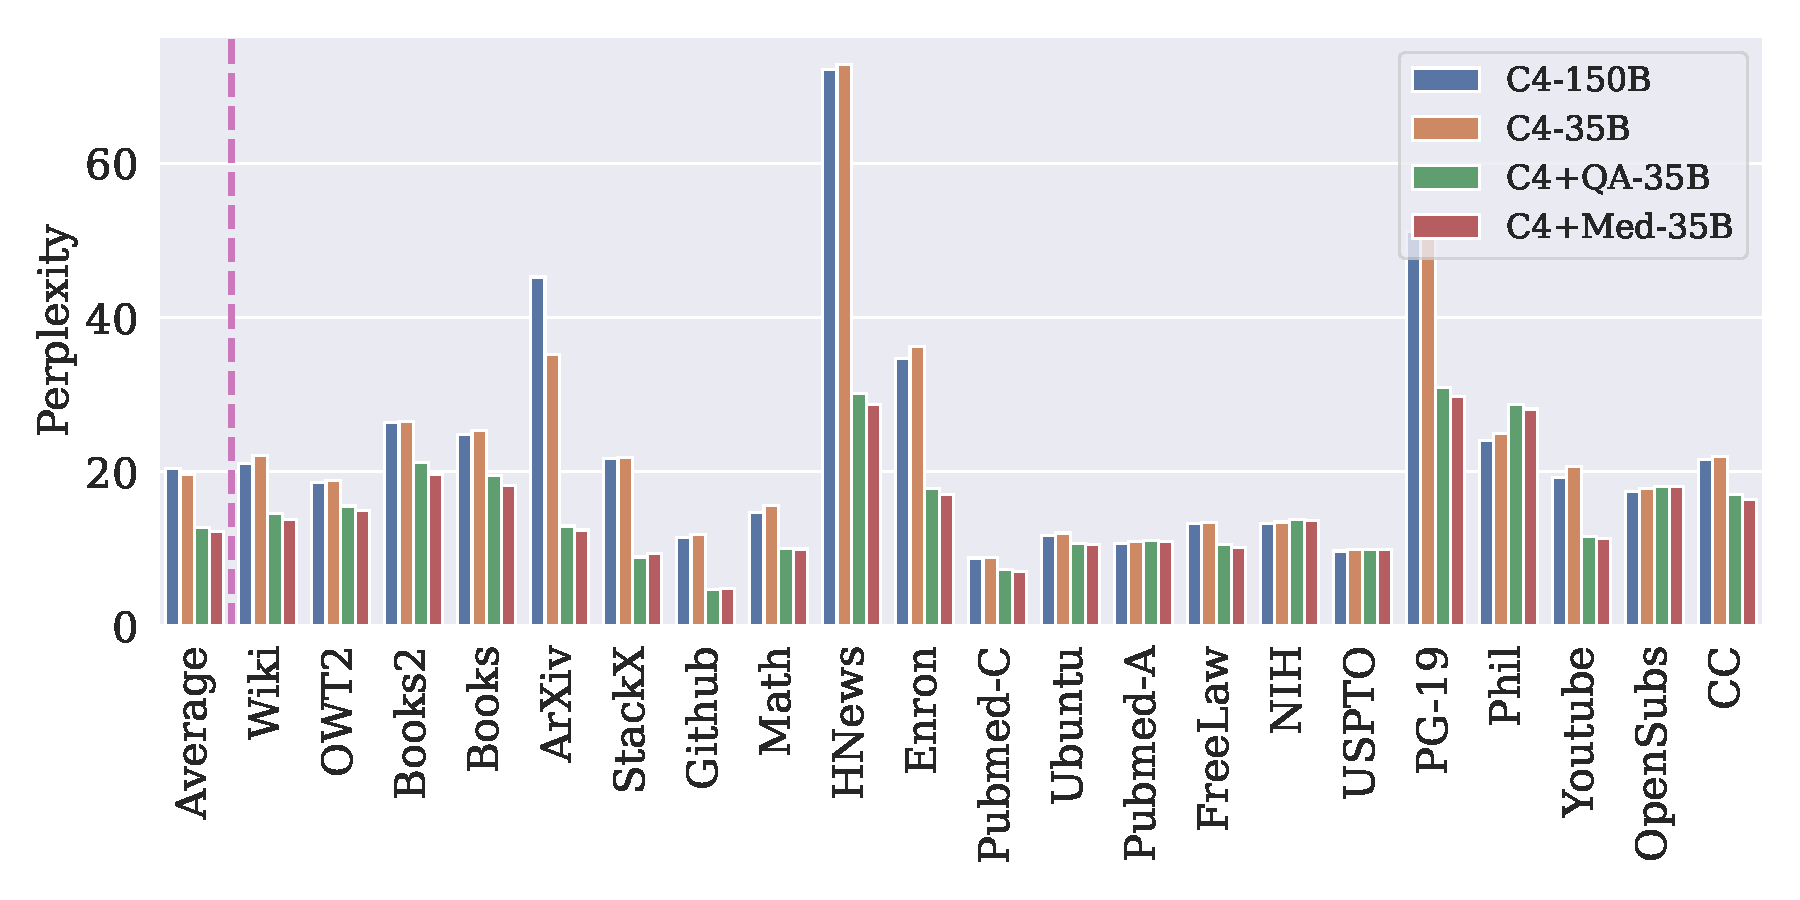
\includegraphics[width=\linewidth]{figures/all_pile_style_1.3B_150k.pdf}
\caption{Perplexity across all domains of the Pile comparing combining multiple styles of synthetic data.  Models are 350M parameters trained for a total of 75B tokens.}
\label{fig:all_perplexity_150k}
\end{figure}


\begin{table*}[t]
    \centering
    \scalebox{0.8}{
    \begin{tabular}{lccccc>{\columncolor{LightCyan}}c}
        \toprule
        Dataset (Real Tok.) & ARC-C & SciQ & PubMedQA & MathQA & MMLU & Avg \\
        \midrule
        C4-35B &  27.0  &  83.4  &  55.0  &  22.5  &  24.3  &  42.4\\
        C4-150B  &  25.9  &  83.8  &  55.4  &  23.5  &  25.4  &  42.8\\
       Med+C4-35B & 27.2  &  82.2  &  46.2  &  23.1  &  25.2  &  40.8\\
        QA+C4-35B & 29.0  &  85.1  &  62.2  &  22.5  &  26.1  &  45.0\\
        \bottomrule
    \end{tabular}}
    \caption{Evaluation of $\sim1.3$B parameter LLMs trained for 150B tokens on Specialized Knowledge Tasks. This table presents the performance on tasks that require specific domain knowledge such as science, medicine, mathematics, and logic.}
    \label{tab:specialized_knowledge_150B}
\end{table*}


\begin{table*}[t]
    \centering
    \scalebox{0.8}{
    \begin{tabular}{lcccccccc>{\columncolor{LightCyan}}c}
        \toprule
        Dataset (Real Tok.) & ARC-E & BoolQ & Wino. & PIQA & HellaSwag & TruthfulQA & OBQA & LogiQA & Avg \\
        \midrule
        C4-35B &  58.6  &  55.2  &  56.1  &  73.9  &  44.5  &  36.0  &  22.2  &  22.8  &  46.2\\
        C4-150B &  59.1  &  54.4  &  56.4  &  74.5  &  44.9  &  34.3  &  22.2  &  22.1  &  46.0\\
        Med+C4-35B &  59.8  &  57.0  &  55.7  &  74.6  &  44.5  &  36.5  &  23.8  &  21.5  &  46.7\\
        QA+C4-35B &  62.2  &  63.3  &  55.7  &  74.8  &  44.6  &  41.4  &  22.4  &  23.2  &  48.4\\
        \bottomrule
    \end{tabular}}
    \caption{Evaluation of $\sim1.3$B parameter LLMs trained for 150B tokens on General Understanding Tasks. This table shows the performance across various datasets, focusing on general reasoning, language understanding, and common sense comparing training .}
    \label{tab:general_understanding_150B}
\end{table*}

\section{LLM Leaderboard Few-shot Results}
In our main experiments in Section~\ref{sec:results} we demonstrate that LLMs trained with synthetic rephrases are a better backbone for  zero-shot question-answering tasks as the model learns the question-answer format and style during pre-training.  In this section, we show that improvements from pre-training on synthetic rephrases are still present even in few-shot settings where the model has access to test samples.  To study few-shot performance, we evaluate on six tasks present in the OpenLLMLeaderboard\footnote{\url{https://huggingface.co/spaces/HuggingFaceH4/open\_llm\_leaderboard}}:

\begin{enumerate}
    \item ARC-Challenge (25 shot)
    \item HellaSwag (10 shot)
    \item MMLU (5 shot)
    \item Truthful-QA (5 shot)
    \item Winogrande (5 shot)
    \item GSM8k (5 shot)
\end{enumerate}

We evaluate two models trained for 300B and 350B tokens corresponding to roughly 85B and 100B unique C4 tokens respectively.  Our findings show substantial improvements on the ARC-challenge benchmark, and Truthful-QA conssitent in the zero-shot settings and comparable performance across other datasets.  Our models also perform better than the publicly released Falcon-1.3B model trained on the Refined Web dataset, and the Pythia-1.4B model, which was trained on Pile.  

\begin{table*}
    \centering
    \resizebox{\textwidth}{!}{
    \begin{tabular}{lcccccc>{\columncolor{LightCyan}}c}
        \toprule 
     Dataset & ARC  &  Hellaswag  &  MMLU  &  TruthfulQA  &  WinoGrande  &  GSM8K  & Avg \\\midrule
     C4 &  31.7  &  62.1  &  26.7  &  33.4  &  57.9  &  0.9  & 35.5 \\
    Falcon-RW &   35.1  &  63.6  &  25.3  &  36.0  &  62.0  &  0.5  & 37.1 \\
     Pythia-1.4b-Pile &    32.7  &  55.0  & 25.6   & 38.7   &  57.3  &  0.8  & 35.0 \\
     \midrule
     QA+C4-85B (300K) &  36.4  &  60.9  & 25.5  &  40.6  &  59.4  &  0.4  & 37.2\\
     QA+C4-100B (350K) &   35.5 &  60.5  & 26.8 &  40.6  & 61.3   & 0.3   & 37.5 \\
     \bottomrule
    \end{tabular}
    }
    \caption{1.3B 300K LLM Leaderboard Eval. Evaluation is done on a single seed (1234).}
    \label{tab:llm_leaderboard}
\end{table*}



\clearpage

\section{Rephrase Prompt Templates}
\label{app:prompt_styles}
We detail the prompts given to the Mistral-7B model to generate synthetic versions of the C4 dataset in specific styles.  \emph{Note: there are slight variations in the prompt that were used for other frozen LLMs, and no prompt was used for the T5 model.}

\subsection*{Easy Style}
A style designed to generate content understandable by toddlers.
\begin{tcolorbox}[colback=gray!20, colframe=gray!75, rounded corners, sharp corners=northeast, sharp corners=southwest]
\texttt{A chat between a curious user and an artificial intelligence assistant. The assistant gives helpful, detailed, and polite answers to the questions. USER: For the following paragraph give me a paraphrase of the same using a very small vocabulary and extremely simple sentences that a toddler will understand:}
\end{tcolorbox}

\subsection*{Hard Style}
A style designed to generate content comprehensible primarily to scholars using arcane language.
\begin{tcolorbox}[colback=gray!20, colframe=gray!75, rounded corners, sharp corners=northeast, sharp corners=southwest]
\texttt{A chat between a curious user and an artificial intelligence assistant. The assistant gives helpful, detailed, and polite answers to the questions. USER: For the following paragraph give me a paraphrase of the same using very terse and abstruse language that only an erudite scholar will understand. Replace simple words and phrases with rare and complex ones:}
\end{tcolorbox}

\subsection*{Medium Style}
A style designed to generate content comparable to standard encyclopedic entries.
\begin{tcolorbox}[colback=gray!20, colframe=gray!75, rounded corners, sharp corners=northeast, sharp corners=southwest]
\texttt{A chat between a curious user and an artificial intelligence assistant. The assistant gives helpful, detailed, and polite answers to the questions. USER: For the following paragraph give me a diverse paraphrase of the same in high quality English language as in sentences on Wikipedia:}
\end{tcolorbox}

\subsection*{Q/A Style}
A style intended to convert narratives into a conversational format.
\begin{tcolorbox}[colback=gray!20, colframe=gray!75, rounded corners, sharp corners=northeast, sharp corners=southwest]
\texttt{A chat between a curious user and an artificial intelligence assistant. The assistant gives helpful, detailed, and polite answers to the questions. USER: Convert the following paragraph into a conversational format with multiple tags of "Question:" followed by "Answer:":}
\end{tcolorbox}

\clearpage

\section{Rephrase Examples}
\textbf{Samplesfrom the MRPC corpus generated by the Mistral-7B model.}

\subsection*{Original}
\begin{tcolorbox}[colback=gray!20, colframe=gray!75, rounded corners, sharp corners=northeast, sharp corners=southwest]
\texttt{The stock rose \$2.11, or about 11 percent, to close Friday at \$21.51 on the New York Stock Exchange.\\\\
    Revenue in the first quarter of the year dropped 15 percent from the same period a year earlier.}
\end{tcolorbox}

\subsection*{Medium Style}
\begin{tcolorbox}[colback=gray!20, colframe=gray!75, rounded corners, sharp corners=northeast, sharp corners=southwest]
\texttt{The stock experienced an increase of approximately 11 percent, closing at \$21.51 on the New York Stock Exchange on Friday, with a rise of \$2.11.\\\\
During the initial three months of the current year, there was a 15 percent decrease in revenue compared to the corresponding quarter of the previous year.}
\end{tcolorbox}

\subsection*{Q/A Style}
\begin{tcolorbox}[colback=gray!20, colframe=gray!75, rounded corners, sharp corners=northeast, sharp corners=southwest]
\texttt{Question: What was the stock's closing price on Friday? Answer: \$21.51 Question: How much did the stock rise on Friday? Answer: \$2.11 or about 11 percent.\\\\
Question: What was the revenue drop in the first quarter compared to the same period last year? Answer: The revenue dropped 15 percent.}
\end{tcolorbox}

\clearpage

\textbf{Samples from the C4 corpus generated by the Mistral-7B model.}

\subsection*{Original}
\begin{tcolorbox}[colback=gray!20, colframe=gray!75, rounded corners, sharp corners=northeast, sharp corners=southwest]
\texttt{First round on stress at work survey. Answering the questionnaire is voluntary and all answers will be saved anonymously. Please fill in this questionnaire only if you have some work experience, part-or full time. Otherwise, you will not be able to answer some of the questions! Here is a the link to all language version.\\\\
Not that there's a thing wrong with frozen burgers. The key here is the meat seasonings, which are pretty strong and spicy and just GOOD, something else I think is really necessary in a turkey burger because ground turkey otherwise can be kind of flavorless. You'll need ground turkey, onion powder, chili powder, salt, pepper, and cayenne pepper for the burgers. Then the mayo takes garlic and onion. Then we need buns, clearly, swiss cheese, lettuce, and onion. I LOVE tomatoes but sometimes find that they get in the way of other flavors, so I left them off of this burger. Add them if you'd like to your array of toppings! First, we'll make the mayo. Grate the garlic directly into the mayo, add a pinch of salt, and squeeze in the lemon juice. Stir. Done! I love this. Then, we'll work on the burgers. Preheat a large skillet to medium-high heat with some olive oil, preheat the broiler to high, then add all the spices to the ground turkey.\\\\
Whether you like your velvet crushed, vibrant or head-to-toe, there's really no denying the sheer luxe and elegance of this timeless textile. Not only is it super stylish, it can actually be so wearable for day-to-day wear. Yes, really! This year it's all about embracing fun gem-toned velvety pieces. Long gone are the days when velvet was solely associated with dark moody shades of navy and black. Below we've rounded up the most covetable velvet pieces on the high street right now. We're already coming up with outfit ideas! Are you completely obsessed or beyond bored of it?\\\\
Save up to \$8,086 on one of 1,258 Chrysler 200s near you. Find your perfect car with Edmunds expert and consumer car reviews, dealer reviews, car comparisons and pricing tools. We have 4,850,420. Research 2015 Chrysler 200 Sedan 4D 200C I4 prices, used values \& 200 Sedan 4D 200C I4 pricing, specs and more. Many years ago, we wrote about the stalling problem with the 2011 Chrysler 200, and believe it or not, we still receive an occasional call regarding the problem.However, a much larger issue has monopolized the phone lines as of late 2015 Chrysler 200 transmission problems leaving drivers with check engine lights, harsh shifting, and the occasional loss of power. The 2015 Chrysler 200 can fetch a premium for its style and its horsepower--but rear-seat room and handling are better bargains elsewhere. Find out why the 2015 Chrysler 200 is rated 8.4 by The. Don't know where to find the perfect rims for your 2015 Chrysler 200 CARiD.com stores a massive selection of 2015 Chrysler 200 wheels offered in myriads of design and finish options, including chrome, black, silver, and so much more.}
\end{tcolorbox}

\clearpage

\subsection*{Medium Style}
\begin{tcolorbox}[colback=gray!20, colframe=gray!75, rounded corners, sharp corners=northeast, sharp corners=southwest]
\texttt{In the initial stage of the survey on work-related stress, participation is optional, and all responses will be kept confidential. It is important to note that only those with work experience, whether part-time or full-time, will be able to accurately respond to certain questions. To complete the questionnaire, please use the following link, which is available in multiple languages.\\\\
Frozen burgers are not inherently flawed, but the meat seasonings are a crucial element that elevates the flavor of the dish. Ground turkey can be quite bland without the right blend of spices, so it is essential to add onion powder, chili powder, salt, pepper, and cayenne pepper to the mixture. Additionally, garlic and onion should be used in the mayonnaise, which is necessary for the burger's topping. To make the mayo, grate the garlic directly into the mixture, add a pinch of salt, and squeeze in lemon juice. Mix well. The mayonnaise is a delicious addition to the burger topping. Now, let's work on the burgers. Heat a large skillet over medium-high heat with some olive oil, and preheat the broiler to high. Add the seasonings to the ground turkey and mix well. The burgers should be cooked on the skillet for about 5 minutes on each side, then transferred to the broiler to cook for an additional 2-3 minutes. The burgers are ready to be assembled on buns, along with swiss cheese, lettuce, and onion. Tomatoes can be added as a topping, but they may overpower other flavors. It is up to the individual to decide if they want to include them in their burger. In conclusion, frozen burgers can be tasty, but the meat seasonings are essential to add depth and flavor to the dish. The mayonnaise and toppings can also be customized to suit individual preferences.\\\\
The luxurious and elegant nature of velvet cannot be denied, whether it is crushed, vibrant, or head-to-toe. This timeless textile is not only fashionable but also wearable for daily wear. In recent years, there has been a shift towards embracing fun gem-toned velvety pieces, breaking away from the traditional association of velvet with dark moody shades of navy and black. Below are some of the most desirable velvet pieces available on the high street today, and we are already envisioning outfits around them. Are you completely enamored with velvet or simply beyond bored with it?\\\\
Discover savings up to \$8,086 on one of 1,258 Chrysler 200s near you. Get expert and consumer car reviews, dealer reviews, car comparisons, and pricing tools from Edmunds. We have 4,850,420 listings for 2015 Chrysler 200 Sedan 4D 200C I4 prices, used values, and more. While we wrote about the stalling problem with the 2011 Chrysler 200, we still receive occasional calls regarding the issue. However, a more significant issue has taken over the phone lines recently - 2015 Chrysler 200 transmission problems that leave drivers with check engine lights, harsh shifting, and occasional loss of power. Despite the premium price for its style and horsepower, rear-seat room and handling are better bargains elsewhere. The 2015 Chrysler 200 is rated 8.4 by The Car Connection. If you're looking for the perfect rims for your 2015 Chrysler 200 CARiD.com offers a vast selection of 2015 Chrysler 200 wheels in various design and finish options, including chrome, black, silver, and more}
\end{tcolorbox}

\clearpage

\subsection*{Q/A Style}
\begin{tcolorbox}[colback=gray!20, colframe=gray!75, rounded corners, sharp corners=northeast, sharp corners=southwest]
\texttt{Question: Is participating in the stress at work survey mandatory? Answer: No, it is voluntary. Question: Will all answers be saved anonymously? Answer: Yes, they will. Question: Who is eligible to take the questionnaire? Answer: Only individuals with work experience, whether part-time or full-time. Question: What happens if someone is not eligible to take the questionnaire? Answer: They will not be able to answer some of the questions. Question: Can you provide a link to all language versions of the questionnaire? Answer: Yes, here is the link.\\\\
Question: What makes these frozen burgers so good? Answer: The meat seasonings are strong and spicy, and they give the burgers a good flavor. Question: Do you think ground turkey can be flavorless? Answer: Yes, ground turkey can be flavorless, but adding spices and seasonings can help. Question: What do you need to make these turkey burgers? Answer: Ground turkey, onion powder, chili powder, salt, pepper, and cayenne pepper for the burgers. Then the mayo takes garlic and onion. Buns, swiss cheese, lettuce, and onion are also needed. Question: What about toppings? Answer: Add tomatoes if you'd like to your array of toppings. Question: How do you make the mayo? Answer: Grate the garlic directly into the mayo, add a pinch of salt, and squeeze in the lemon juice. Stir. Done! Question: How do you work on the burgers? Answer: Preheat a large skillet to medium-high heat with some olive oil, preheat the broiler to high, then add all the spices to the ground turkey.\\\\
Question: What do you think of velvet? Answer: Whether you like your velvet crushed, vibrant or head-to-toe, there's really no denying the sheer luxe and elegance of this timeless textile. Question: Is velvet super stylish? Answer: Yes, really! This year it's all about embracing fun gem-toned velvety pieces. Question: Was velvet solely associated with dark moody shades of navy and black? Answer: Long gone are the days when velvet was solely associated with dark moody shades of navy and black. Question: Do you have any covetable velvet pieces on the high street right now? Answer: Below we've rounded up the most covetable velvet pieces on the high street right now. Question: Are you completely obsessed or beyond bored of it? Answer: We're already coming up with outfit ideas!\\\\
Question: How can I save money on a Chrysler 200? Answer: Save up to \$8,086 on one of 1,258 Chrysler 200s near you. Find your perfect car with Edmunds expert and consumer car reviews, dealer reviews, car comparisons and pricing tools. Question: What are the problems with the 2015 Chrysler 200? Answer: We have 4,850,420. Research 2015 Chrysler 200 Sedan 4D 200C I4 prices, used values \& 200 Sedan 4D 200C I4 pricing, specs and more. Many years ago, we wrote about the stalling problem with the 2011 Chrysler 200, and believe it or not, we still receive an occasional call regarding the problem. However, a much larger issue has monopolized the phone lines as of late 2015 Chrysler 200 transmission problems leaving drivers with check engine lights, harsh shifting, and the occasional loss of power. Question: What are the benefits of buying a 2015 Chrysler 200? Answer: The 2015 Chrysler 200 can fetch a premium for its style and its horsepower--but rear-seat room and handling are better bargains elsewhere. Question: How is the 2015 Chrysler 200 rated? Answer: It's rated 8.4 by The. Question: Where can I find the perfect rims for my 2015 Chrysler 200? Answer: CARiD.com stores a massive selection of 2015 Chrysler 200 wheels offered in myriads of design and finish options, including chrome, black, silver, and so much more.}
\end{tcolorbox}


